\chapter{\selectlanguage{greek}Θεωρητικό υπόβαθρο}
\begin{itemize}
\item περιγραφή πειράματος και
\item Για να καταλάβει ο κόσμος τι σημαίνει
\item Γιατί είναι χρήσιμο
\item Φωτογραφίες
\item Τι χρειάζεται να ξέρω
\item Το πείραμα
\end{itemize}

Στο κεφάλαιο αυτό παρουσιάζονται αναλυτικά οι 

\section{\selectlanguage{greek}Το \en{CERN}}

To \en{CERN}, διατηρώντας το ακρωνύμιο της αρχικής Γαλλικής ονομασίας του \en{$``$Conseil Européen pour la Recherche Nucléaire$"$}, είναι το μεγαλύτερο σε έκταση πειραματικό κέντρο πυρηνικών ερευνών και ειδικότερα επί της σωματιδιακής φυσικής στον κόσμο. 
Βρίσκεται δυτικά της Γενεύης, στα σύνορα Ελβετίας και Γαλλίας και ιδρύθηκε το 1954 από 12 ευρωπαϊκές χώρες. 
Σήμερα αριθμεί 20 κράτη-μέλη, μεταξύ των οποίων και η Ελλάδα, η οποία είναι και ιδρυτικό μέλος.

\begin{figure}[h]

\includegraphics[width=0.25\textwidth]{images/CERNlogo.png}
\centering
\caption{Το λογότυπο του \en{CERN}}
\label{img:CERNlogo}
\end{figure}

Η βασική λειτουργία του \en{CERN} είναι η παροχή επιταχυντών σωματιδίων και άλλων υποδομών απαραίτητων για την έρευνα στον τομέα της φυσικής υψηλών ενεργειών και ως αποτέλεσμα έχουν πραγματοποιηθεί πολυάριθμα πειράματα στο \en{CERN} μέσω διεθνών συνεργασιών.

Επίσης, το \en{CERN} αποτελεί τη γενέτειρα του Παγκόσμιου Ιστού (\en{World Wide Web}).
Στην κύρια τοποθεσία του στο \en{Meyrin} βρίσκεται μεγάλη εγκατάσταση ηλεκτρονικών υπολογιστών με ισχυρές υποδομές επεξεργασίας δεδομένων, κυρίως για την ανάλυση των πειραματικών δεδομένων. 
Λόγω της ανάγκης να καταστούν αυτές διαθέσιμες σε εξωτερικούς ερευνητές, υπήρξε ιστορικά ένας σημαντικός κόμβος δικτύου ευρείας περιοχής (\en{Wide Area Network}).

Αρκετά σημαντικά επιτεύγματα στο πεδίο της φυσικής των σωματιδίων έγιναν μέσω πειραμάτων στο \en{CERN}. Αυτά περιλαμβάνουν:
\begin{itemize}
\item 1973: Ανακάλυψη των ουδέτερων ρευμάτων στο θάλαμο φυσαλίδων \en{Gargamelle}.
\item 1983: Ανακάλυψη των μποζονίων $W$ και $Z$ στα πειράματα \en{UA1} και \en{UA2}.
\item 1995: Πρώτη δημιουργία ατόμων αντιυδρογόνου στο πείραμα \en{PS210}.
\item 1999: Ανακάλυψη της άμεσης παραβίασης \en{CP} στο πείραμα \en{NA48}.
\item 2010: Απομόνωση 38 ατόμων αντιυδρογόνου.
\item 2011: Διατήρηση αντιυδρογόνου για πάνω από 15 λεπτά.
\item 2012: Ένα μποζόνιο με μάζα περίπου \SI[per-mode = symbol]{125}{\GeV \per  \clight \squared} συνάδει με τον πολυπόθητο μποζόνιο \en{Higgs}.
\end{itemize}


\section{\selectlanguage{greek}Ο επιταχυντής \en{CLIC}}


Ο \en{CLIC -- Compact Linear Collider} -- αποτελεί μια μελέτη για ένα μελλοντικό επιταχυντή που θα φτάσει σε πρωτοφανή επίπεδα ενέργειας ηλεκτρόνια και αντισωμάτιά τους, ποζιτρόνια. 
Όταν θα έρχονται σε επαφή μέσω σύγκρουσης, θα καταστρέφουν το ένα το άλλο, απελευθερώνοντας όλη τους την ενέργεια για την παραγωγή νέων σωματιδίων.

\begin{figure}[b]

\includegraphics[width=0.25\textwidth]{images/CLIClogo}
\centering
\caption{Το λογότυπο του \en{CLIC}}
\label{img:CLIClogo}
\end{figure}

Τα ηλεκτρόνια και τα ποζιτρόνια είναι θεμελιώδη σωματίδια και οι συγκρούσεις τους μπορούν να προσφέρουν εξαιρετικά λεπτομερείς πληροφορίες σχετικά με τους νόμους της φύσης. 
Έτσι ο \en{CLIC} θα προσφέρει σημαντικές θεμελιώδεις γνώσεις φυσικής, πέρα από αυτές που είναι διαθέσιμες από το Μεγάλο Επιταχυντή Αδρονίων (\en{Large Hadron Collider -- LHC}) ή από ένα γραμμικό επιταχυντή ηλεκτρονίων/ποζιτρονίων χαμηλότερης ενέργειας, λόγω του μοναδικού συνδυασμού πειραματικής ακρίβειας και υψηλής ενέργειας.

Σε αυτές τις υψηλές ενέργειες, τα ηλεκτρόνια και ποζιτρόνια θα έχαναν ένα τεράστιο μέρος της ενέργειάς τους επιταχυνόμενα σε έναν κυκλικό επιταχυντή σαν τον \en{LHC}. 
Έτσι, τα σωματίδια πρέπει να επιταχυνθούν σε δύο γραμμικούς επιταχυντές που αντικρίζουν ο ένας τον άλλο, έτσι ώστε οι δέσμες να συγκρούονται στον κεντρικό ανιχνευτή. 
Αυτό συνεπάγεται ότι τα σωματίδια πρέπει να αποκτήσουν την ενέργειά τους από ένα και μόνο πέρασμα τους μέσα από τις κοιλότητες επιτάχυνσης.

\begin{figure}[h]
\includegraphics[width=0.5\textwidth]{images/CLIC-twobeam.jpg}
\centering
\caption{Το σύστημα δύο δεσμών του \en{CLIC}}
\label{img:CLICtwobeamscheme}
\end{figure}

Ο \en{CLIC} έχει σχεδιαστεί για να κατασκευαστεί σε στάδια αυξανόμενης ενέργειας για σύγκρουση: ξεκινώντας από \SI{360}{\GeV}, περίπου \SI{1.4}{\TeV}, και μέχρι την τελική ενέργεια των \SI{3}{\TeV}. 
Προκειμένου να επιτευχθεί αυτή η ενέργεια με ένα ρεαλιστικό και οικονομικά αποδοτικό τρόπο, η αύξηση της επιτάχυνσης πρέπει να είναι πολύ υψηλή.
Ο \en{CLIC} αποσκοπεί σε επιτάχυνση των \SI[per-mode = symbol]{100}{\mega \volt \per \metre}, 20 φορές υψηλότερη από αυτή του \en{LHC}.

Αυτή η δέσμη-οδηγός (\en{drive beam}) επιβραδύνεται σε ειδικές Διατάξεις Εξαγωγής και Mεταφοράς Ισχύος -- \en{Power Extraction and Transfer Structures (PETS)}, και η παραγόμενη \en{RF} ισχύς μεταφέρεται στην κύρια δέσμη. 
Αυτό οδηγεί σε μια πολύ απλή διάταξη σήραγγας χωρίς ενεργά \en{RF} μέρη (δηλ. \en{klystrons}).

\begin{figure}[h]
\includegraphics[width=\textwidth]{images/CLIC-layout.jpg}
\centering
\caption{Το σχεδιάγραμμα του \en{CLIC}}
\label{img:CLIClayout}
\end{figure}

\begin{figure}[h]
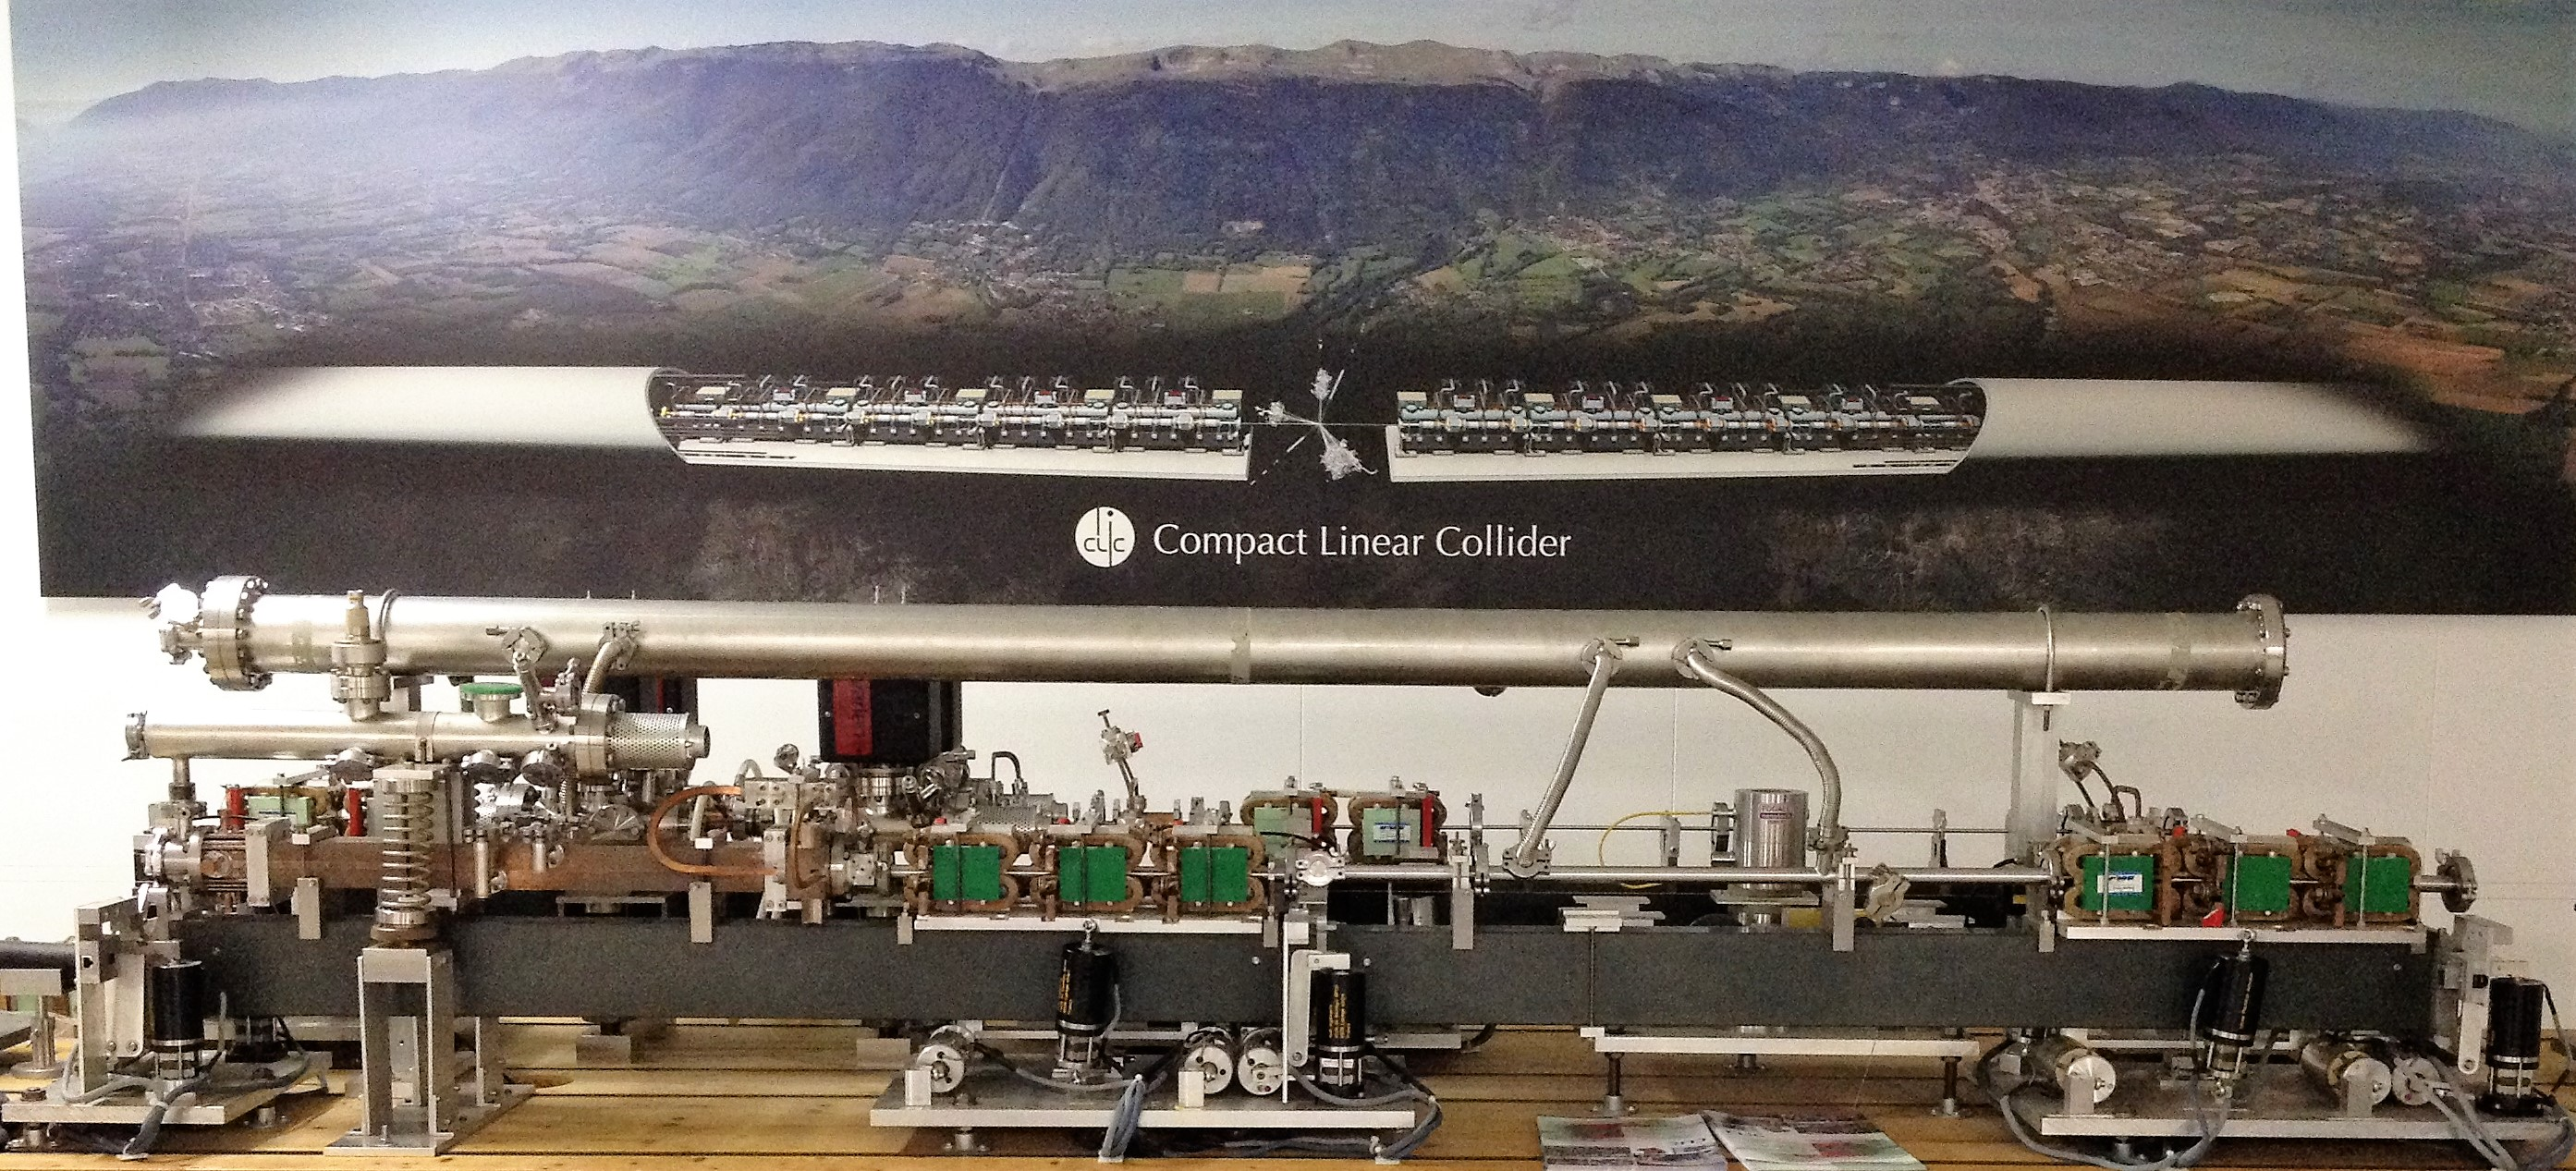
\includegraphics[width=\textwidth]{images/CLIC-maquette}
\centering
\caption{Η μακέτα του \en{CLIC} που βρίσκεται στο κτήριο δοκιμών \en{CLIC Test Facility 3 (CTF3)} του \en{CERN}}
\label{img:CLIClmaquette}
\end{figure}

Ο \en{CLIC} είναι μία από τις επιλογές για έναν μελλοντική επιταχυντή κατασκευασμένο στο \en{CERN}. Η τελική απόφαση κατασκευής θα εξαρτηθεί από τα μελλοντικά αποτελέσματα του \en{LHC}.

\begin{figure}[h]
    \begin{subfigure}{0.5\textwidth}
		\centering
		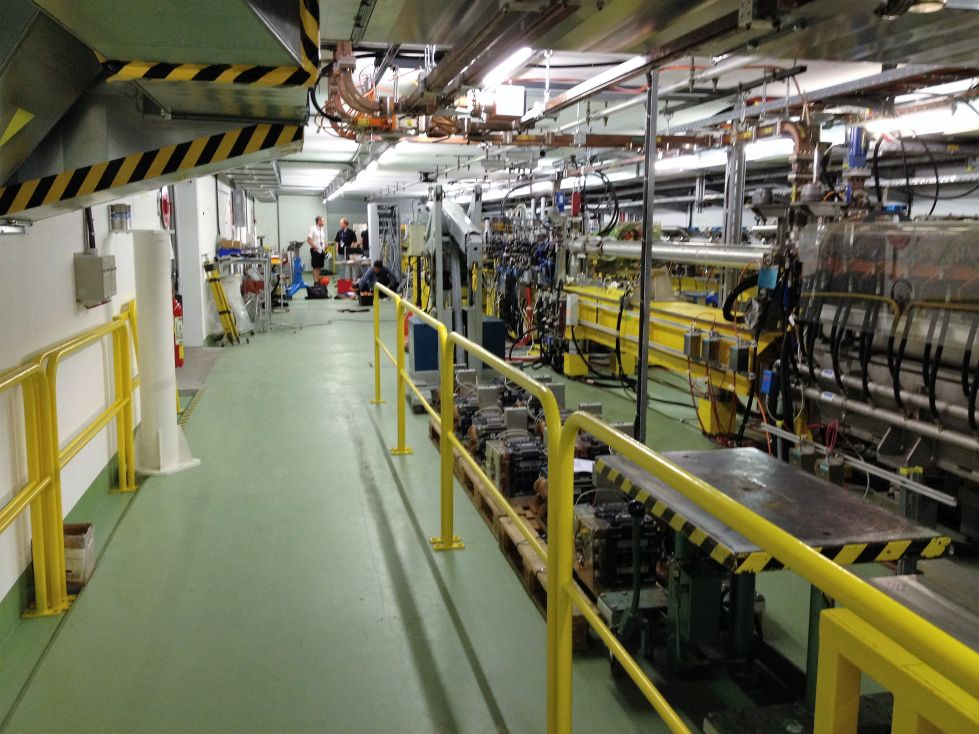
\includegraphics[width=.9\linewidth]{images/CLIC-CTF3-overview.jpg}
    \end{subfigure}
	~
    \begin{subfigure}{0.5\textwidth}
		\centering
		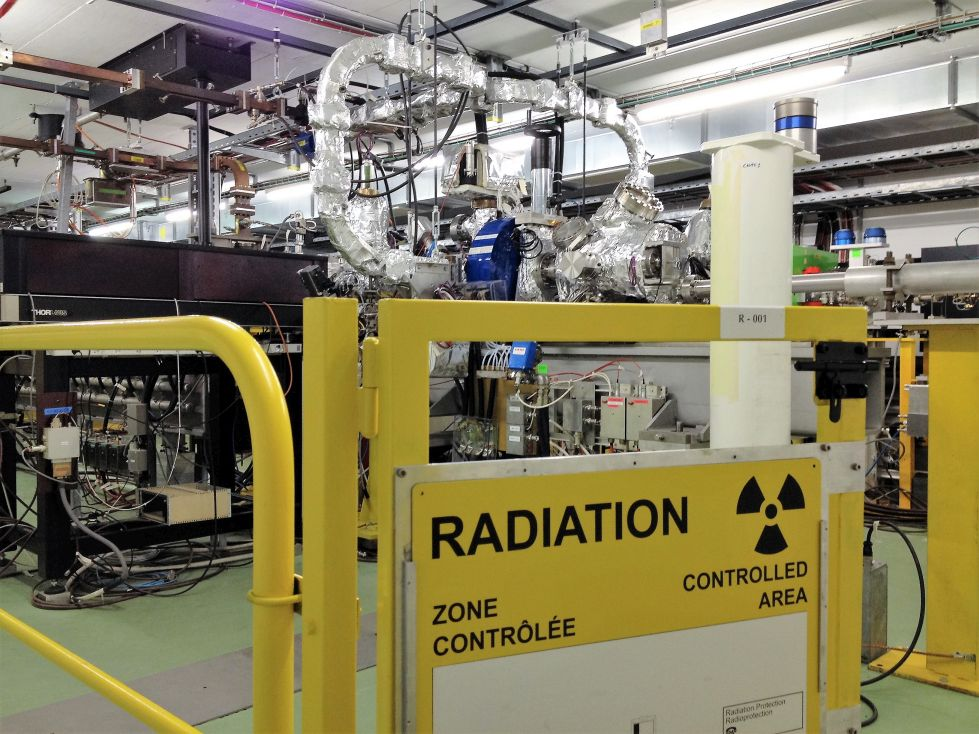
\includegraphics[width=.9\linewidth]{images/CLIC-CTF3-radiation.jpg}
    \end{subfigure}
	\par\bigskip
    \begin{subfigure}{0.5\textwidth}
		\centering
		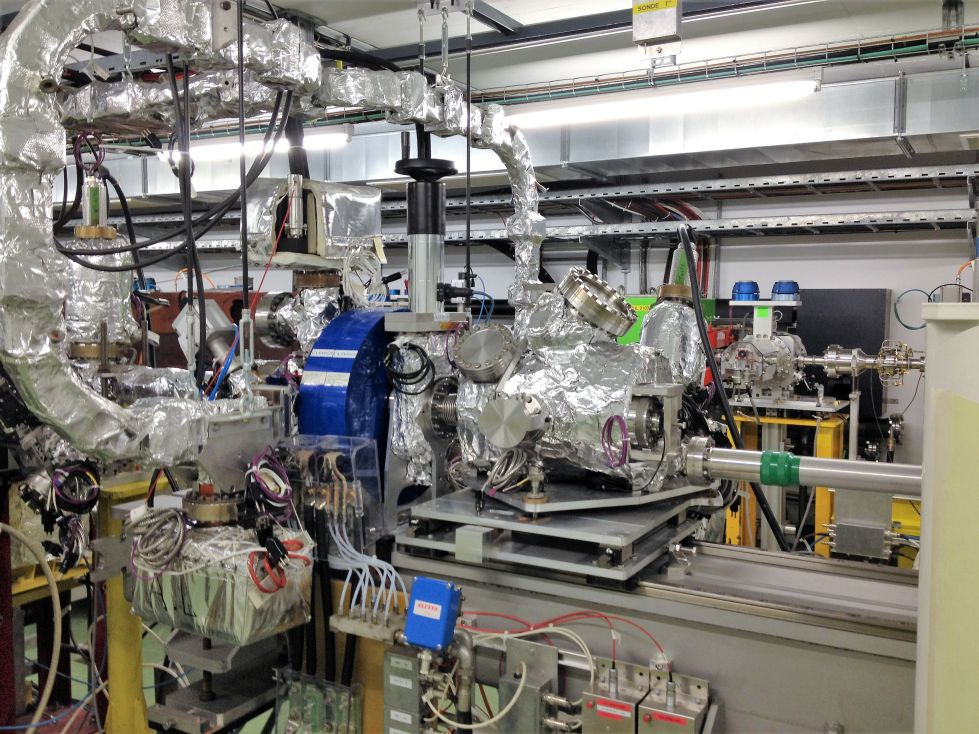
\includegraphics[width=.9\linewidth]{images/CLIC-CTF3-img1.jpg}
    \end{subfigure}        
	~
    \begin{subfigure}{0.5\textwidth}
		\centering
		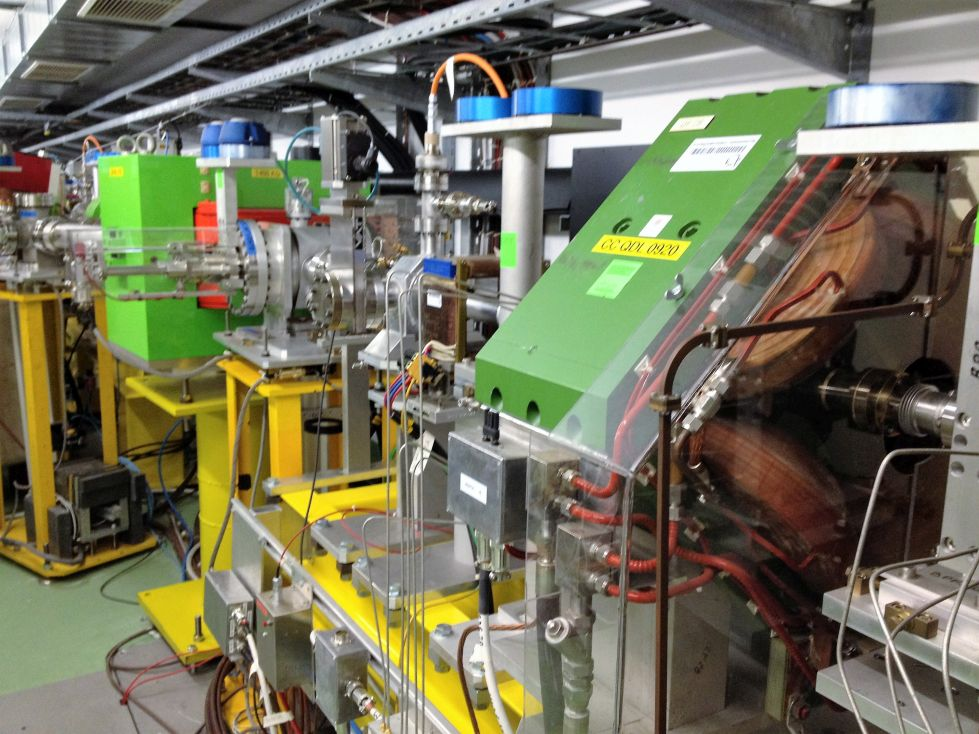
\includegraphics[width=.9\linewidth]{images/CLIC-CTF3-img2.jpg}
    \end{subfigure}
	\par\bigskip
    \begin{subfigure}{0.5\textwidth}
		\centering
		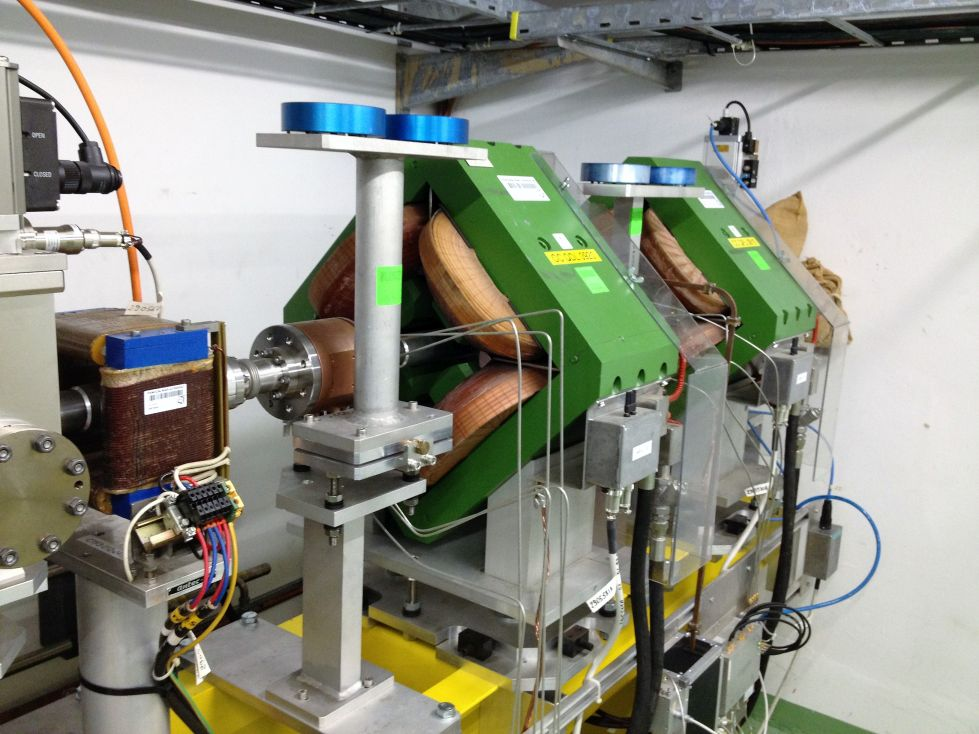
\includegraphics[width=.9\linewidth]{images/CLIC-CTF3-img3.jpg}
    \end{subfigure}        
	~
    \begin{subfigure}{0.5\textwidth}
		\centering
		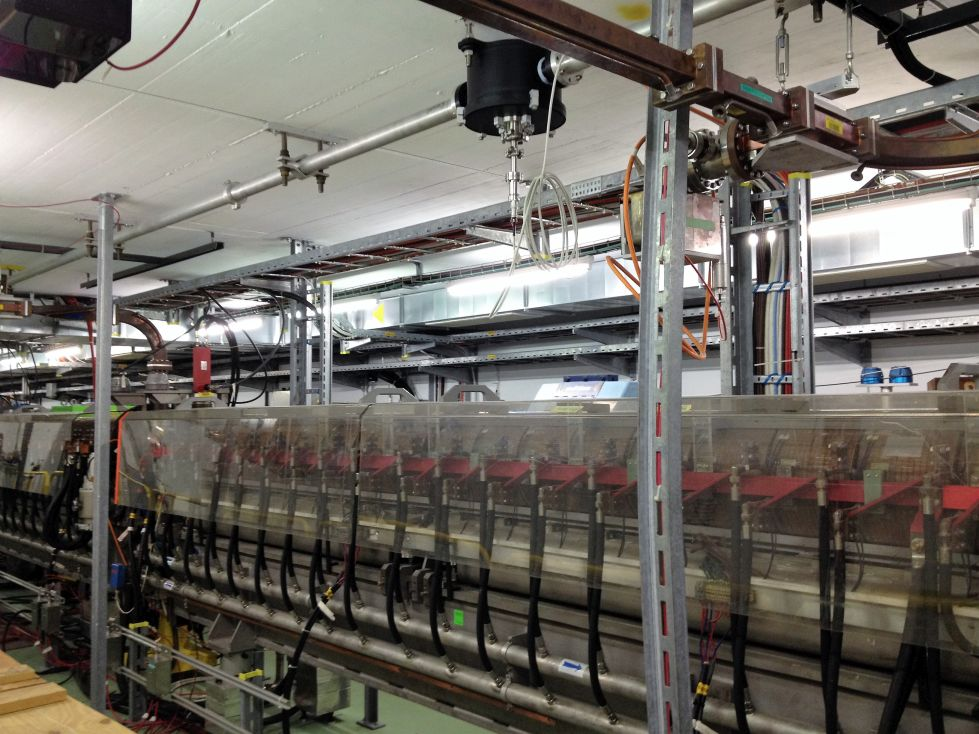
\includegraphics[width=.9\linewidth]{images/CLIC-CTF3-img4.jpg}
    \end{subfigure}
    
\caption[Εικόνες από το \en{CLIC Testing Facility 3}]{Εικόνες από το \en{CLIC Testing Facility 3 (CTF3)}, όπου γίνονται δοκιμές για το \en{CLIC}. Λόγω της φύσης των δοκιμών, το \en{CTF3} θεωρείται \en{$``$radiation controlled zone$"$} και για την είσοδο κάποιου στο χώρο απαιτείται να έχει περάσει 7-ωρη εκπαίδευση (\en{radiation training}) και να φέρει ειδικό δοσίμετρο κατά την επίσκεψη}
\label{img:CLIC-CTF3}        
\end{figure}

\section{\selectlanguage{greek}Το \en{Electron beam scanner}}

$$\theta_y (x) = \frac{2 \rho r_e}{\beta} \int_{-\infty}^{\infty}\frac{n(z) \mathrm{d}z}{\rho^2 + \left(x+\beta z \right) ^2}$$

$$\theta_z(x) = 2 r_e \int_{-\infty}^{\infty}\frac{(x+\beta z)n(z) \mathrm{d}z}{\rho^2 + \left(x+\beta z \right) ^2}$$